\documentclass[../../main.tex]{subfiles}

\begin{document}

\subsection*{Grundlagen der Gruppentheorie}
\pagecolor{violet!20}
Ganz zu Beginn dieses Buchs hast du dich mit den Grundrechenarten beschäftigt -- erst hast du ausschließlich mit natürlichen Zahlen gerechnet und dann hast du den Zahlbereich immer weiter ausgebaut -- über die ganzen Zahlen bis hin zu den rationalen und schließĺich den reellen Zahlen. Die vier Grundrechenarten, die dir bekannt sind, heißen Addition, Subtraktion, Multiplikation und Division.

Du weißt, dass für die Addition und die Multiplikation das \textbf{Kommutativgesetz} und das \textbf{Assoziativgesetz} gilt. Es gibt noch ein paar weitere Dinge, die vermutlich ziemlich selbstverständlich für dich sind: Wenn du 0 zu irgendeiner anderen Zahl addierst, veränderst du die Zahl dadurch nicht: Es gilt $a+0=a$ für alle Zahlen $a$. Auch für die Multiplikation gilt so etwas ähnliches: $a\cdot 1=a$. Die Zahl 0 wird daher auch das \textbf{neutrale Element der Addition} genannt -- und die 1 ist das \textbf{neutrale Element der Multiplikation}. Die Bezeichnung \emph{neutral} kommt daher, dass die Auswirkung der Addition von 0 neutral für den Wert des Terms ist (da es ihn ja nicht verändert). Seitdem du Brüche kennst, kannst du auch mit dem Begriff des Kehrwerts etwas anfangen. Für einen Bruch $\frac{a}{b}$ ($a$ und $b$ seien hier ganze Zahlen) ist der Kehrwert $\frac{b}{a}$. Multiplizierst du die beiden Brüche, kannst du das Ergebnis letztlich zu 1 kürzen -- also zum neutralen Element der Multiplikation. Natürlich kannst du zu jedem Bruch den Kehrwert bilden (denn du musst einfach immer nur den Zähler und Nenner vertauschen). Folglich findest du zu jedem Bruch $p$ einen zweiten Bruch $q$, sodass deren Produkt $pq=1$ ist. Ein ähnliches Phänomen kennst du auch für die Addition: Für eine Zahl $a$ ist die Gegenzahl $-a$ und es gilt $a+(-a)=a-a=0$ (also erhältst du auch hier wieder das neutrale Element). Der Kehrwert bzw. die Gegenzahl werden auch als \textbf{inverse Elemente} bezeichnet, weil sie genau das Gegenteil einer Zahl darstellen und weil sie sich gegenseitig aufheben.

\begin{advexample}{}
    Die Zahl $7$ wird mit $6$ multipliziert, um $42$ zu erhalten. Um von der $42$ zur $7$ zurück zu kommen, muss die Multiplikation mit $6$ rückgängig gemacht werden. Das inverse Element zur $6$ ist ihr Kehrwert, also $\frac{1}{6}$. Tatsächlich gilt $42\cdot \frac{1}{6}=\frac{42}{6}=7$. Ansonsten hättest du vermutlich einfach $42:6$ gerechnet. Die Idee an dieser Stelle ist es, dass wir auf dem Hinweg die gleiche Rechenart wie auf dem Rückweg verwenden wollen.
\end{advexample}

\begin{advexample}{}
    Der Term $x+18$ soll so verändert werden, dass nur noch $x$ übrig bleibt. Dass auf das $x$ der Wert 18 addiert wird, lässt sich mit dem \emph{inversen Element} der 18, also der $-18$, wieder rückgängig machen: $x+18+(-18)=x+0=x$. Das Addieren von $-18$ macht das Addieren von $18$ also rückgängig.
\end{advexample}

Tatsächlich brauchen wir also eigentlich überhaupt keine Subtraktion oder Division. Alles, was wir je gerechnet haben, können wir ausschließlich mithilfe der Addition und Multiplikation ausdrücken, wenn wir die beiden folgenden Regeln anwenden:
\begin{align*}
    a-b=a+(-b)~\text{und}~a:b=a\cdot \frac{1}{b}
\end{align*}

Die Idee der Gruppentheorie ist es, dass wir solche Zusammenhänge (also, dass sich mehrere auf den ersten Blick verschiedene Vorgänge eigentlich genau gleich verhalten) besser verstehen wollen. Es zeigt sich nämlich, dass sich diese Eigenschaften (also Assoziativität, neutrale Elemente und inverse Elemente) nicht nur bei der Addition und Multiplikation herkömmlicher Zahlen finden lassen, sondern auch bei vielen weiteren Beispielen, die wir uns gleich anschauen. Um nicht jedes Mal von vorn anzufangen, nutzt die Gruppentheorie diese Gemeinsamkeiten aus und ermöglicht es, Aussagen zu treffen, die allgemein für jede Struktur zutreffen, die die oben genannten Eigenschaften besitzt. Für Strukturen, die diese Eigenschaften haben, hat man den Namen \textbf{Gruppe} vergeben.

Bevor wir uns anschauen, was eine Gruppe in der Mathematik ist, schauen wir uns einmal an, was die Addition eigentlich genau macht. Das ist nicht weiter schwierig: Wir haben zwei Zahlen, addieren sie und erhalten als Ergebnis die Summe. Genauer gesagt bekommen wir zwei Zahlen aus einer bestimmten Menge, etwa zwei ganze Zahlen. Und natürlich sollte auch die Summe dann wieder eine ganze Zahl sein. Wir könnten nun also eine Funktion $f$ definieren, die zwei ganze Zahlen erhält und sie addiert:
\[f\colon \Integer\times\Integer, f(a,b)=a+b.\]
\begin{advexample}{}
    Es gilt $5+9=14$. Die Funktion $f$ erhält als Argument zwei Zahlen, also beispielsweise die 5 und die 9, und es gilt $f(5,9)=5+9$, also $f(5,9)=14$. Damit macht die Funktion $f$ genau dasselbe wie die normale Addition. Theoretisch ließe sich eine Rechnung wie $1+2+3$ auch als $(1+2)+3=f(1,2)+3=f(f(1,2),3)$ schreiben.
\end{advexample}
Um sofort zu sehen, dass die Funktion eigentlich nur zwei Zahlen addiert, könnten wir sie auch $+$ nennen, denn Funktionen können ja beliebig benannt werden. In diesem Fall erhalten wir die Funktion $+$ und schreiben $+(a,b)=a+b$. Für die Multiplikation könnten wir eine Funktion $*$ mit $*(a,b)=ab$ definieren. Wir fassen einmal zusammen, was wir gerade gemacht haben:
\begin{itemize}
    \item Wir haben eine Menge (die ganzen Zahlen \Integer) gewählt, deren Elemente wir addieren möchten.
    \item Wir haben eine Funktion definiert, die zwei Elemente $a$ und $b$ unserer Menge \Integer{} nimmt und zu ihrer Summe $a+b$ verknüpft.
    \item Weil wir es gewohnt sind, schreiben wir $a+b$ statt $+(a,b)$. 
    \item Die Funktion ist wegen $(a+b)+c=a+(b+c)$ assoziativ. In Funktionenschreibweise heißt das $+(+(a,b),c)=+(a,+(b,c))$.
    \item Es gibt eine Zahl, die wir zu jeder anderen Zahl $a$ addieren können, ohne $a$ zu verändern: Die Zahl 0.
    \item Wir können zu jeder beliebigen Zahl $a$ eine andere Zahl, nämlich $-a$, finden, sodass ihre Summe 0 ist.
\end{itemize}
Mit anderen Worten: Die Addition ist nichts anderes als eine Funktion auf den ganzen Zahlen (ebenso natürlich die Multiplikation).

Die hier genannten Eigenschaften sind genau das, was wir allgemein von einer Gruppe fordern. Auch eine Gruppe wird im Wesentlichen durch eine Rechenoperation ausgemacht, die für Elemente (hier Zahlen) einer bestimmten Menge funktioniert. Wenn wir die oben genannten Eigenschaften von einer Kombination aus einer Rechenoperation $*$ und einer Menge $G$ fordern, dann machen wir das formal wie in der folgenden Definition.

\begin{definition}{Gruppe}
    Eine \textbf{Gruppe} ist ein Tupel $(G,*)$, bestehend aus einer Menge $G$ und einer Funktion $*\colon G\times G\rightarrow G$ (genannt \textbf{Verknüpfung} auf $G$) mit $*(a,b)=a*b$ für beliebige $a,b \in G$, wobei gilt:
    \begin{enumerate}
        \item[(G1)] Die Verknüpfung $*$ ist \emph{assoziativ}, d.h. $(a*b)*c=a*(b*c)$ für alle $a,b,c\in G$.
        \item[(G2)] Es gibt ein \emph{neutrales Element} $e\in G$, sodass $e*g=g*e=0$ für alle $g\in G$.
        \item[(G3)] Zu jedem Element $g\in G$ existiert ein \emph{inverses Element} $g^{-1}\in G$, sodass $g*g^{-1}=g^{-1}*g=e$ gilt.
    \end{enumerate}
\end{definition}
\begin{advexample}{}
    Die ganzen Zahlen \Integer{} sind eine Gruppe bezüglich der Addition. Wie bereits bekannt ist, gilt für die Addition nämlich das Assoziativgesetz. Außerdem ist 0 das neutrale Element der Addition und $-a$ ist das inverse Element zu einem beliebigen $a\in\Integer$.
    
    Weil damit alle Axiome abgedeckt sind, ist $(\Integer,+)$ mit $+(a,b)=a+b$ eine Gruppe.
\end{advexample}
Der wesentliche Unterschied zwischen etwas wie der Addition auf den dir bekannten Zahlen und dem Begriff der Gruppe ist, dass eine Gruppe viel allgemeiner ist. Zu Beginn ist das vermutlich sehr verwirrend, weil du dir darunter nicht wirklich etwas vorstellen kannst. Am besten denkst du beim Umgang mit Gruppen daher einfach, du hättest es mit der Addition in den ganzen Zahlen zu tun. Wie im letzten Beispiel erläutert, bilden die ganzen Zahlen nämlich eine Gruppe, wenn man die herkömmliche Addition als seine Verknüpfung auswählt. Doch auch die folgenden Beispiele, die teilweise überhaupt nichts mit der Addition zu tun haben, sind Gruppen.

\begin{advexample}{}
    Wenn wir über die Uhrzeit sprechen, beginnen wir nach Ablauf eines Tages immer wieder von vorn mit dem Zählen der Stunden: Wenn um 23 Uhr noch zwei Stunden vergehen, ist es nicht 25 Uhr, sondern 1 Uhr. Die Uhrzeiten, die wir kennen, lassen sich durch die Zahlen $0,1,2,\dots,23$ darstellen. Statt die Reihe mit $24$ fortzusetzen, fangen wir nach der $23$ wieder bei $0$ an.
    
    Bei der Uhrzeit verwendet man eine sogenannte \textbf{Modulo-Arithmetik}. Das bedeutet, dass man zunächst normal rechnet (etwa $20+7=27$), anschließend aber das Ergebnis solange verkleinert, bis es wieder kleiner als eine Zahl (hier $24$) ist. Das machen wir, indem wir die $27$ mit Rest durch $24$ teilen. Es gilt nämlich $27=1\cdot 24\,R\,3$. Wir nun nur mit dem Rest weiter.
\end{advexample}

\begin{advexample}{}
    \parpic[r]{
        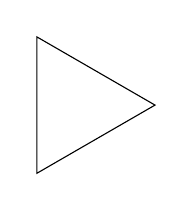
\begin{tikzpicture}
            \draw (0:1) -- (1200:1) -- (240:1) -- cycle;
            \node at (120:1) {\blueball};
            \node at (240:1) {\redball};
            \node at (0:1) {\greenball};
        \end{tikzpicture}
    }
    \picskip{6}
    Du siehst rechts ein gleichseitiges Dreieck. Wir würden das Dreieck gern so drehen, dass es seine Form nicht verändert, also so, dass dort, wo vor der Drehung eine Ecke war, auch nach der Drehung eine Ecke ist. Wir können das Dreieck auf zwei Weisen drehen: Entweder im Uhrzeigersinn oder gegen den Uhrzeigersinn. Alternativ ist es natürlich auch möglich, einfach gar nichts zu machen. Was wir erhalten, ist eine Gruppe, in der wir keine Zahlen verknüpfen, sondern Drehungen eines Dreiecks. Die drei Drehungen überführen das oben abgebildete Dreieck in einer der drei folgenden Positionen:
    \begin{multicols}{3}
        \begin{center}
        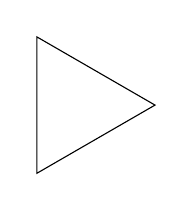
\begin{tikzpicture}
            \draw (0:1) -- (1200:1) -- (240:1) -- cycle;
            \node at (120:1) {\greenball};
            \node at (240:1) {\blueball};
            \node at (0:1) {\redball};
        \end{tikzpicture}
        
        $D_L$: Drehung nach links
        
        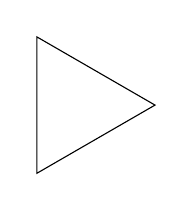
\begin{tikzpicture}
            \draw (0:1) -- (1200:1) -- (240:1) -- cycle;
            \node at (120:1) {\blueball};
            \node at (240:1) {\redball};
            \node at (0:1) {\greenball};
        \end{tikzpicture}
        
        Keine Drehung ($D_0$)
        
        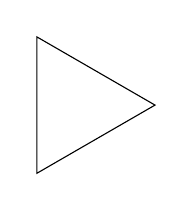
\begin{tikzpicture}
            \draw (0:1) -- (1200:1) -- (240:1) -- cycle;
            \node at (120:1) {\redball};
            \node at (240:1) {\greenball};
            \node at (0:1) {\blueball};
        \end{tikzpicture}
        
        $D_R$: Drehung nach rechts
        \end{center}
    \end{multicols}
    
    Die Menge der möglichen Drehungen ist $D=\{D_L, D_0, D_R\}$. Diese enthält die Drehung nach links, die Drehung nach rechts und die Möglichkeit, das Dreieck gar nicht zu drehen. Statt das Dreieck nur einmal zu drehen, können wir es auch mehrmals hintereinander drehen, zum Beispiel zweimal nach links. Wir wollen das Hintereinanderausführen von Drehungen mithilfe des Symbols $\circ$ notieren. Das zweimalige Drehen nach links schreiben wir also als $D_L\circ D_L$. Die Frage ist nun, ob wir dasselbe Ergebnis auch mit einer einzigen Drehung hätten erreichen können. Die Antwort ist natürlich ja, denn wir hätten auch einfach einmal nach rechts drehen können. Für zwei Drehungen $D_1,D_2$ soll $D_1\circ D_2$ nun einfach die Drehung sein, mit der wir in einem Schritt das gleiche Ergebnis erreichen wie wenn wir erst $D_1$ und dann $D_2$ ausführen. Es gilt also beispielsweise $D_L\circ D_L=D_R$, weil wir einmal nach rechts drehen können statt zweimal nach links zu drehen.
    
    Die folgende Tabelle zeigt, was passiert, wenn wir zwei Drehungen hintereinander ausführen.
    
    \begin{center}
        \begin{tabular}{c|ccc}
            $\circ$ & $D_0$ & $D_L$ & $D_R$ \\\hline
            $D_0$ & $D_0$ & $D_L$ & $D_R$\\
            $D_L$ & $D_L$ & $D_R$ & $D_0$\\
            $D_R$ & $D_R$ & $D_0$ & $D_L$\\
        \end{tabular}
    \end{center}
        
    Wir können nun überprüfen, dass $(D,\circ)$ eine Gruppe ist. Dafür müssen wir die drei Gruppenaxiome überprüfen.
    \begin{enumerate}
        \item[(G1)] Wir müssen zunächst zeigen, dass Drehungen assoziativ sind, also, dass für beliebige Drehungen $D_1,D_2,D_3\in D$ gilt: $(D_1\circ D_2)\circ D_3=D_1\circ (D_2\circ D_3)$. Hier passiert aber nur das Folgende: Entweder wir führen erst eine Drehung aus, die $D_1$ und $D_2$ entspricht und drehen anschließend noch mithilfe von $D_3$ das Dreieck. Oder wir drehen das Dreieck erst mithilfe von $D_1$ und anschließend mit der Drehung, die entsteht, wenn wir $D_2$ und $D_3$ in einer Drehuns zusammen ausführen. Das ist natürlich genau das gleiche.
        \item[(G2)] Die Drehung $D_0$ verändert das Dreieck nicht. Wenn wir also eine beliebige Drehung $d$ nehmen und anschließend die Drehung $D_0$ ausführen, dann haben wir insgesamt trotzdem nur die Drehung $d$ ausgeführt. Es gilt also $D_0\circ d=d$ und $d\circ D_0=d$. Folglich ist $D_0$ das neutrale Element der Gruppe.
        \item[(G3)] Angenommen, wir haben das Dreieck mithilfe von $D_L, D_R$ oder $D_0$ gedreht. Jetzt müssen wir eine Drehung finden, die wir danach ausführen können, um die Drehung rückgängig zu machen. Das funktioniert ganz einfach: Für $D_0$ müssen wir nichts rückgängig machen, also können wir mithilfe von $D_0$ einfach ein zweites Mal nichts machen (d.h. $D_0^{-1}=D_0$). Haben wir das Dreieck nach links gedreht ($D_L$), dann können wir es anschließend nach rechts drehen $(D_R)$ und haben die Drehung rückgängig gemacht. Also ist $D_L^{-1}=D_R$ und $D_R^{-1}=D_L$.
    \end{enumerate}
    Damit haben wir gezeigt, dass $(D,\circ)$ die Gruppenaxiome erfüllt.
\end{advexample}

\begin{theorem}{Kürzungsregel}
    Es seien $G$ eine Gruppe und $a,b,c \in G$. Dann gilt $a=b$ genau dann, wenn $ac=bc$.
\end{theorem}
\begin{proof}
     Wenn wir drei Elemente $a,b,c \in G$ mit $a=b$ haben, dann gilt natürlich auch $ac=bc$, weil wir $a$ und $b$ beliebig durch einander ersetzen können -- sie sind ja gleich. Wir zeigen als nächstes, dass umgekehrt aus $ac=bc$ folgt, dass auch schon $a$ und $b$ gleich sein müssen (also $a=b$). Wir zeigen also, dass $a=b$ gilt und dürfen dafür verwenden, dass \mbox{$a+c=b+c$ \textcolor{orange!75!black}{$(*)$}} gilt. Das machen wir so:
    \[a\axiom{G2}a\cdot 1\axiom{G3}a\cdot(c\cdot c^{-1})\axiom{G1}(a\cdot c)\cdot c^{-1}\axiom{$*$}(b\cdot c)\cdot c^{-1}\axiom{G1}b\cdot (c\cdot c^{-1})\axiom{G3}b\cdot 1\axiom{G2}b.\]
    Diese Umformung sieht sehr kleinschrittig aus, aber wichtig ist, dass wir in jedem Schritt sicher sind, dass er funktioniert, weil wir hier nur jeweils ein Axiom angewandt haben (das jeweils verwendete Axiom steht immer an den Gleichheitszeichen).
    
\end{proof}

\newpage
\pagecolor{white}

\end{document}